\documentclass{article}

\usepackage{graphicx} % Per immagini

%\setlength\parindent{0pt} % Rimuove indendazioni
\usepackage[utf8x]{inputenc} %serve per i simboli utf8x

\usepackage{times} % Uncomment to use the Times New Roman font
\usepackage{siunitx}
\usepackage{float} %serve per mettere le immagini in posizione Here
\usepackage{subfig} %serve per mettere più figure in colonna o in riga
\usepackage[a4paper,total={170mm,257mm},left=25mm,top=35mm,right=25mm,bottom=35mm]{geometry} % per il layout


\begin{document}

	\title{RELAZIONI DI LABORATORIO DI BIOLOGIA MOLECOLARE}

	\author{Litterini S. \\Giulio B. \\Cracco A.\\Buzzolan T. }

	\date{\today}

	\maketitle

	\vspace{1.5cm}

	\large{\textbf{ELENCO DELLE RELAZIONI :}}
	\vspace{0.5cm}

	\begin{enumerate}

		\item Minipreparazione di DNA plasmidico
		\item Estrazione dell'RNA totale con TRIZOL
		\item Preaparazione TAE 50X e restrizione del DNA
		\item Polymerase Chain Reaction (PCR)
		\item Praparazione terreno LB, cellule competenti e piastre LB-agar
		\item Trasformazione delle cellule di E. coli XL1 Blue
		\item Allestimento culture cellulari
		\item Utilizzo delle culture cellulari umane in analisi molecolari e morfologiche
		\item Estrazione RNA con kit su colonnina Qiagen: Retrotrascrizione in cDNA
		\item Amplificazione RealTime PCR ed Estrazione delle proteine totali
		\item SDS-PAGE delle proteine estratte
		\item Separazione cellulare su gradiente di ficoll

	\end{enumerate}

	\newpage

	%STRUMENTI

	\large{\textbf{STRUMENTI UTILIZZATI NELLE ESPERIENZE :}}

	\begin{enumerate}

		\item Provette Eppendorf :

		\begin{figure}[H]

			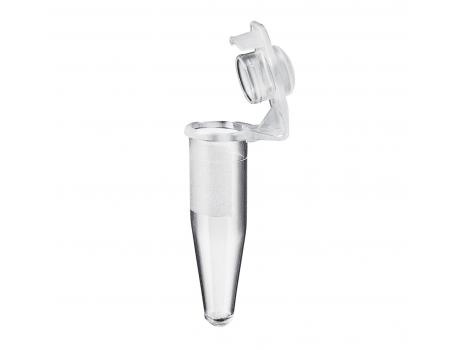
\includegraphics[width=0.6\textwidth]{./immagini/eppendorf.jpg}
			%\caption{provetta Eppendorf}
			\label{eppendorf}

		\end{figure}

		\vspace{0.5cm}


		\item Provette Falcon :

		\begin{figure}[H]

			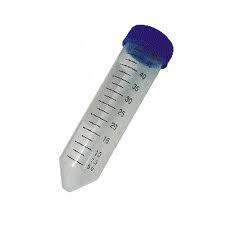
\includegraphics[width=0.6\textwidth]{./immagini/falcon.jpeg}
			%\caption{provetta Falcon}
			\label{falcon}

		\end{figure}

		\vspace{0.5cm}


		\item Micropipette e puntali:

		\begin{figure}[H]

			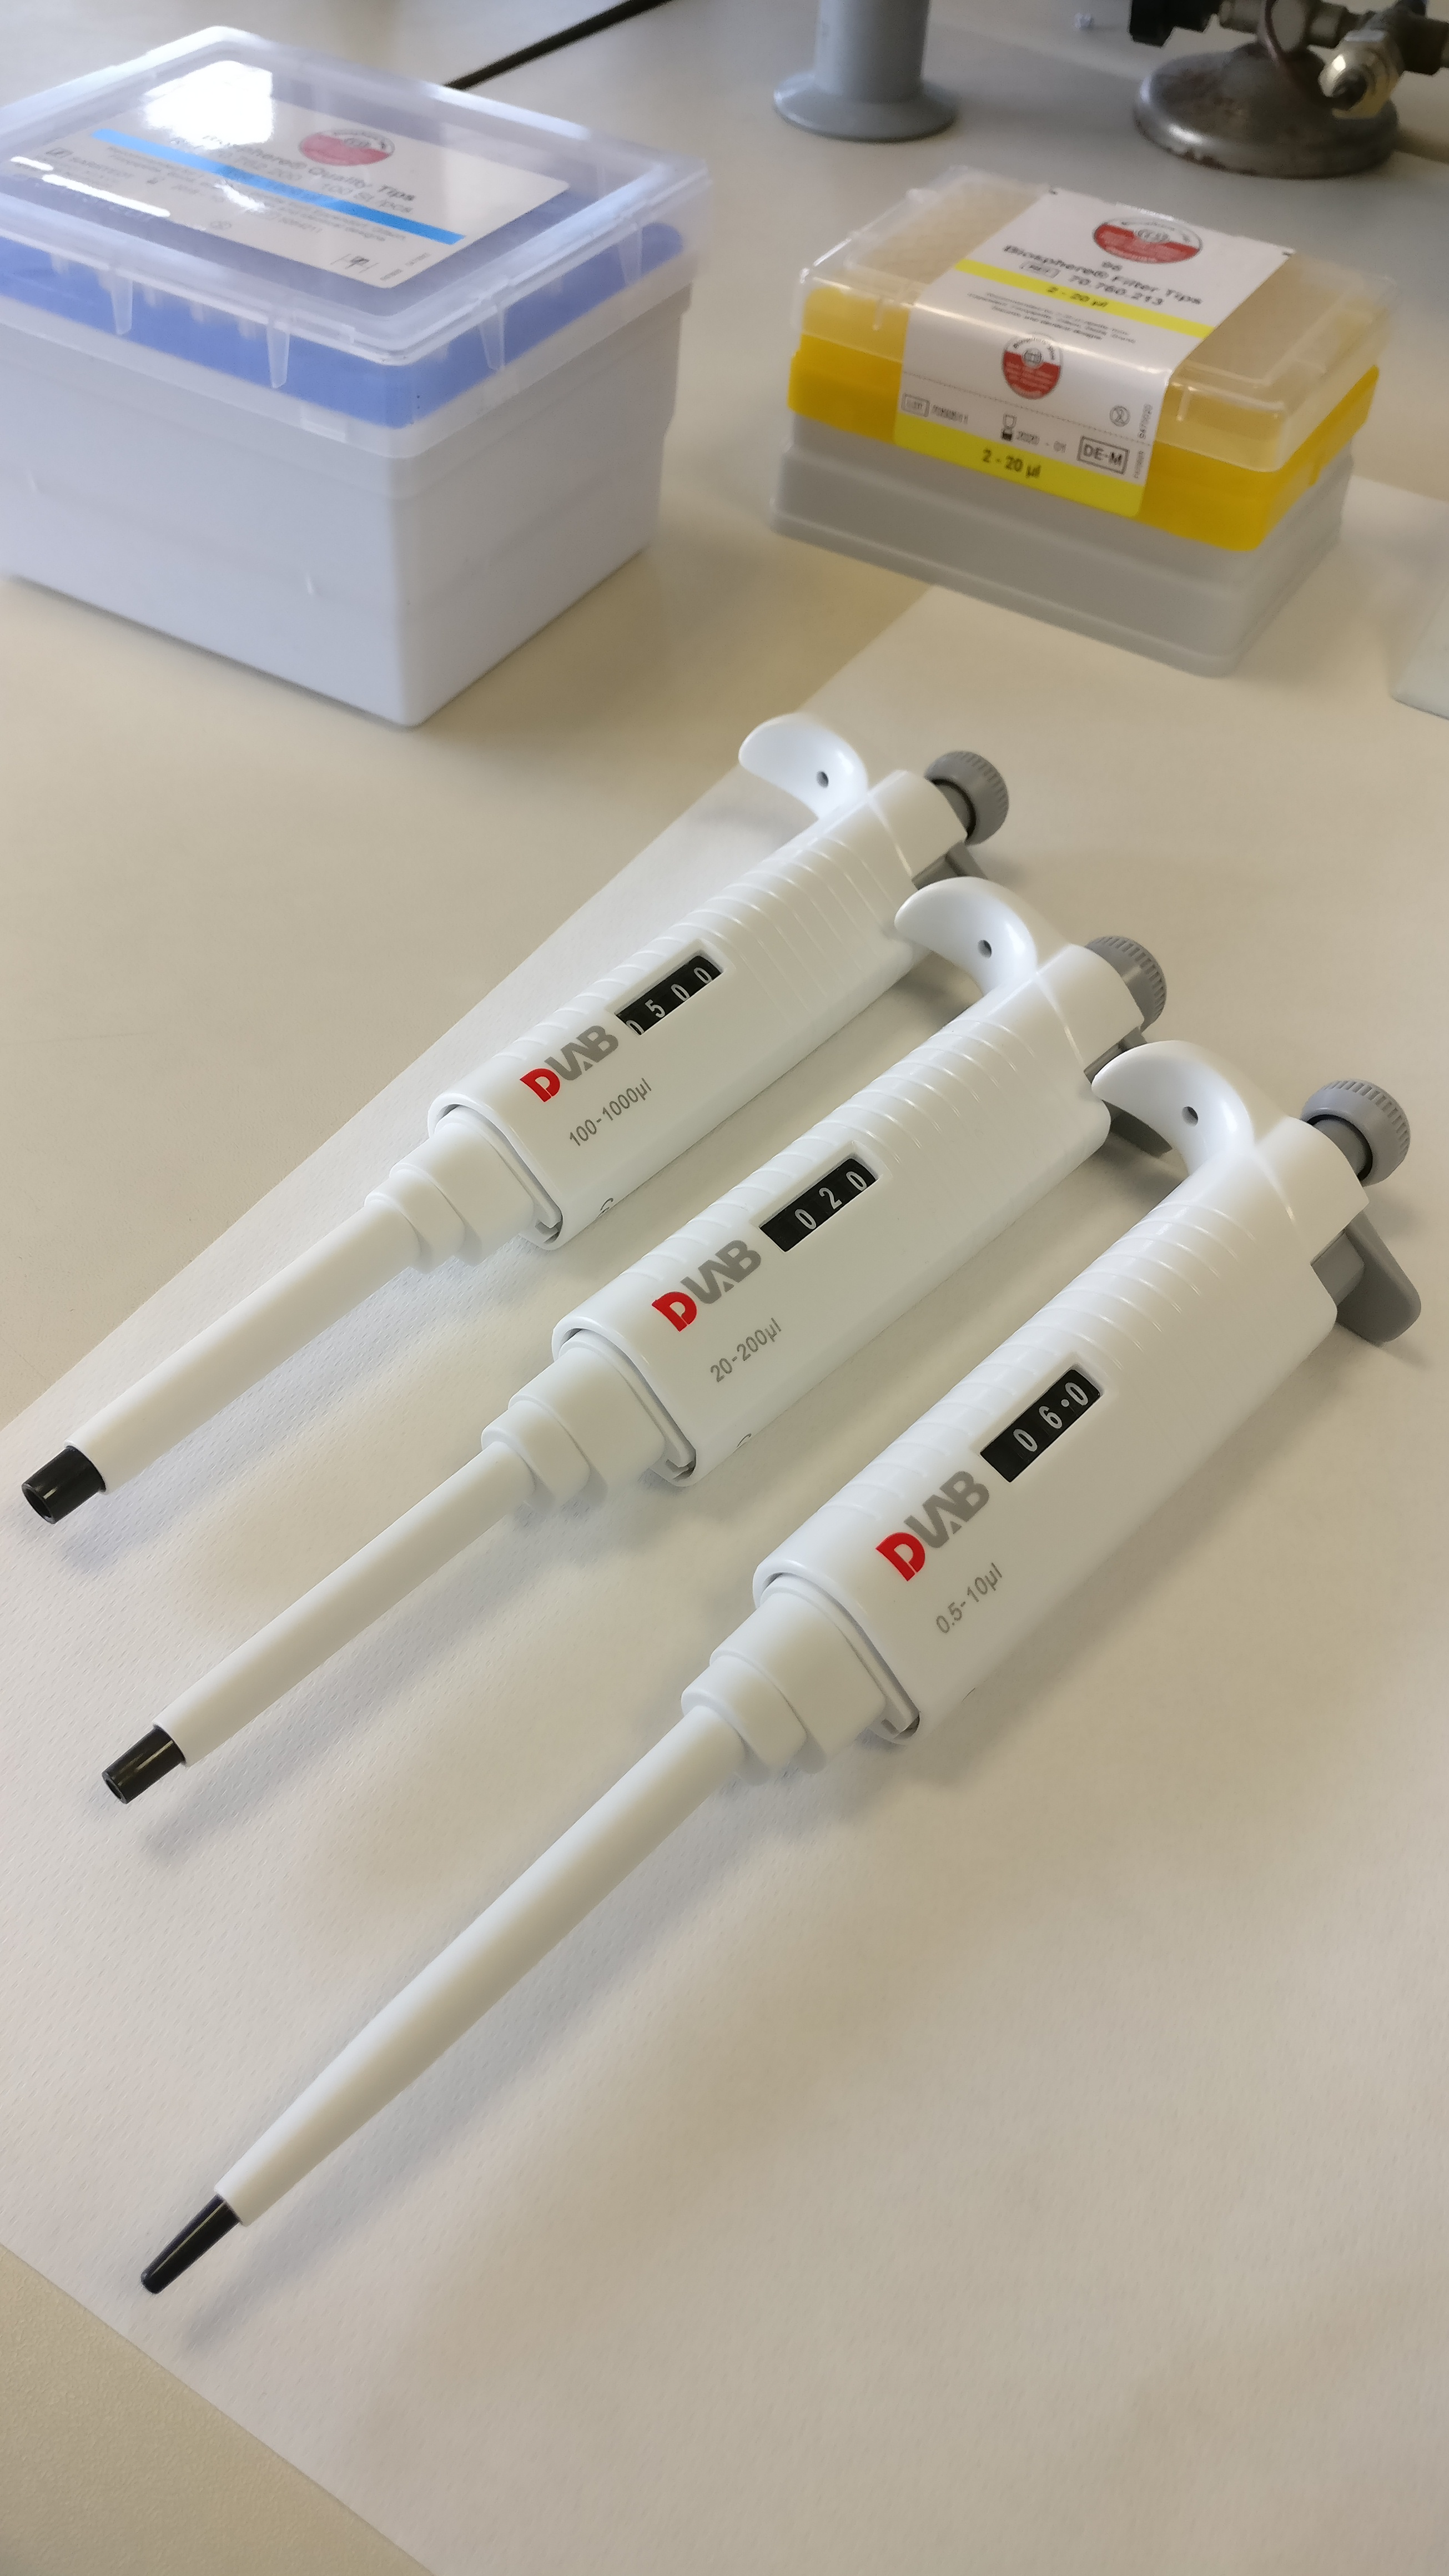
\includegraphics[width=0.35\textwidth]{./immagini/micropipette.jpg}
			%\caption{micropipette e puntali in sfondo}
			\label{micropipette}

		\end{figure}

		\vspace{0.5cm}


		\item Microscopio ottico:

		\begin{figure}[H]

			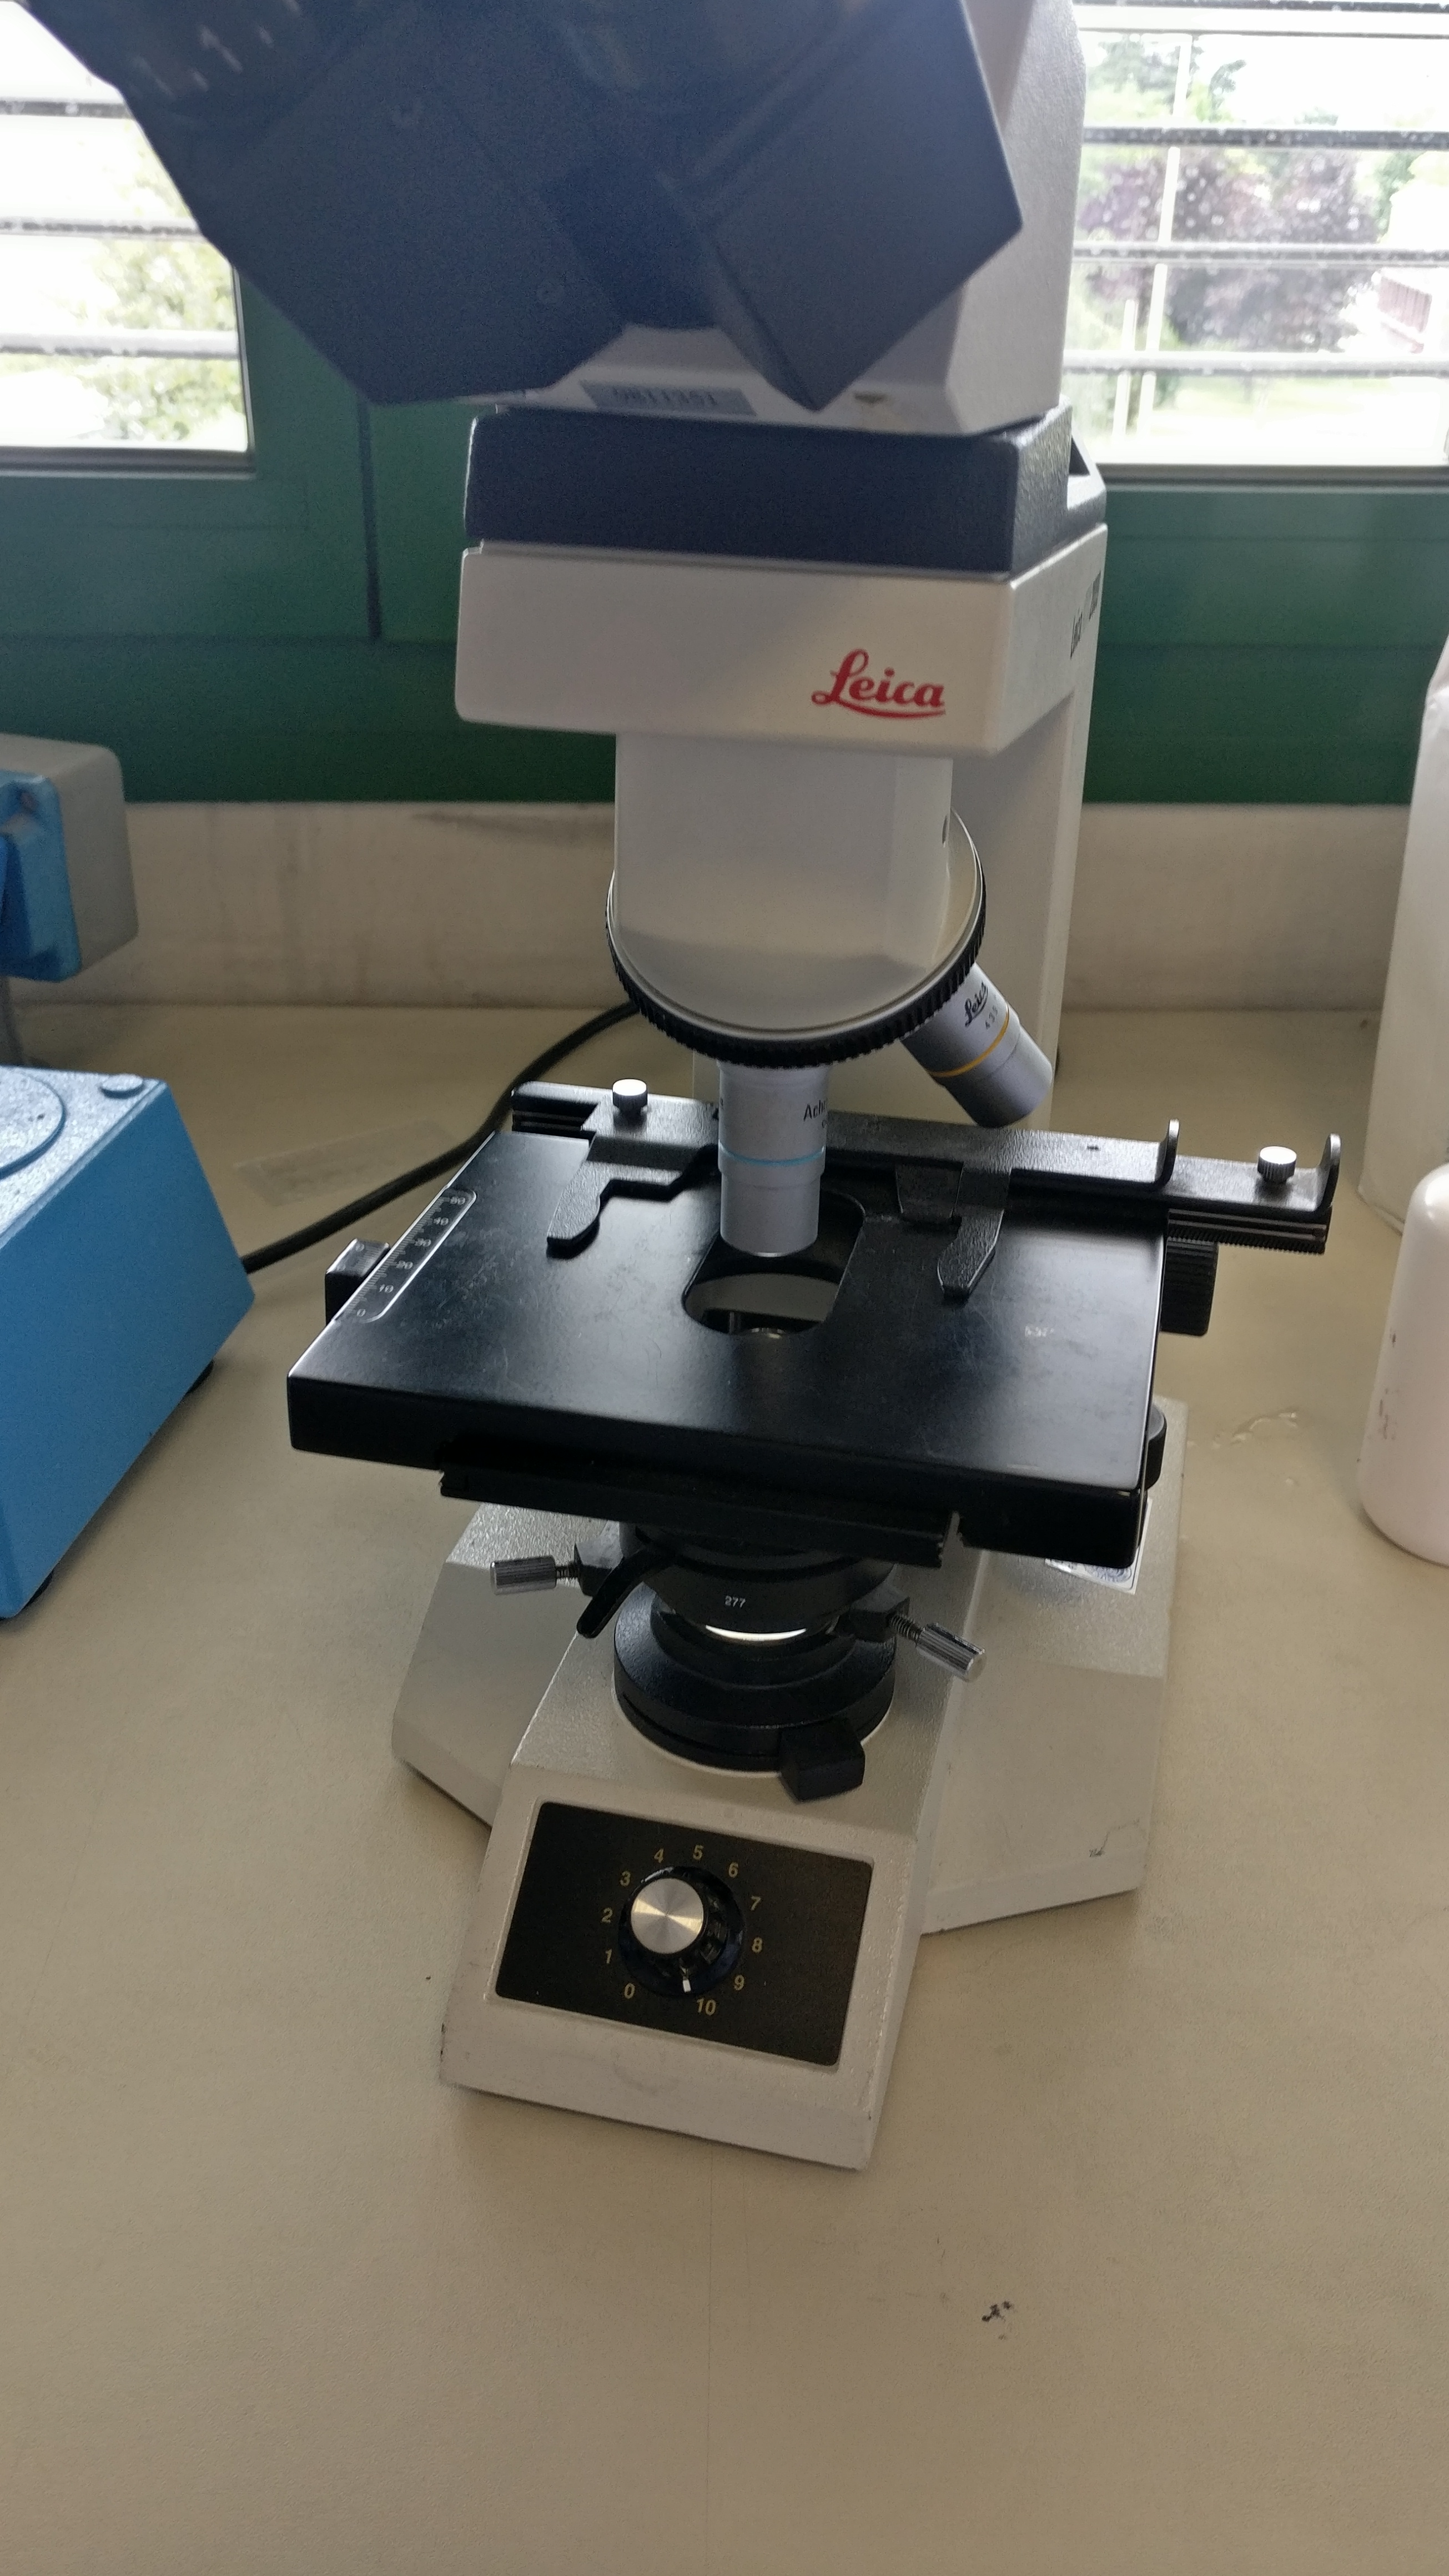
\includegraphics[width=0.35\textwidth]{./immagini/microscopio.jpg}
			%\caption{microscopio ottico}
			\label{microscopio}

		\end{figure}

		\vspace{0.5cm}


		\item guanti in lattice:

		\begin{figure}[H]

			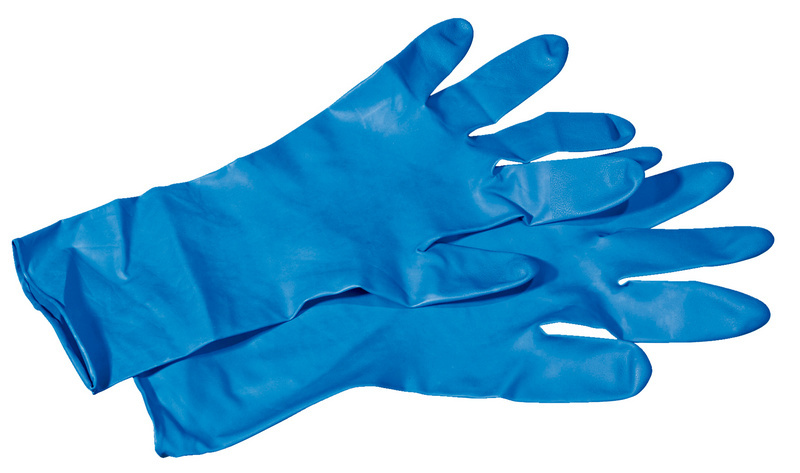
\includegraphics[width=0.5\textwidth]{./immagini/guanti.jpg}
			%\caption{Guanti in lattice da laboratorio}
			\label{guanti}

		\end{figure}

		\vspace{0.5cm}


		\item Camice:

		\begin{figure}[H]

			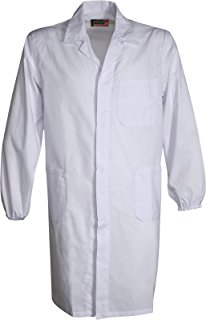
\includegraphics[width=0.4\textwidth]{./immagini/camice.jpg}
			%\caption{Camice da laboratorio}
			\label{camice}

		\end{figure}

		\vspace{0.5cm}


		\item Beuta:

		\begin{figure}[H]

			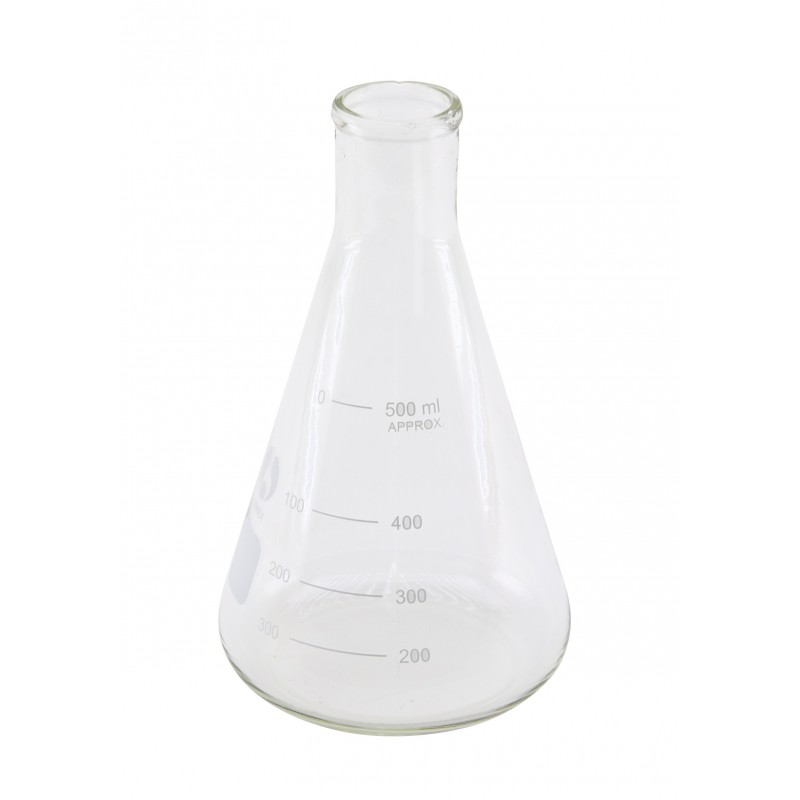
\includegraphics[width=0.5\textwidth]{./immagini/beuta.jpg}
			%\caption{Camice da laboratorio}
			\label{camice}

		\end{figure}

		\vspace{0.5cm}


		\item Vasca per l'elettroforesi:

		\begin{figure}[H]

			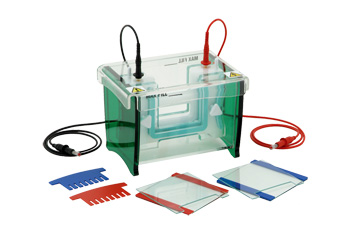
\includegraphics[width=0.7\textwidth]{./immagini/vasca_elettroforesi.jpg}
			\label{vasca_elettroforesi}

		\end{figure}

		\vspace{0.5cm}

	\end{enumerate}


	\newpage
	%_______________________________ESPERIENZA N° 3 (ELETTROFORESI)
	\section{\LARGE{Preparazione TAE e Restrizione del DNA}}

\vspace{0.6cm}


\subsection{Sommario}

\subsubsection{Scopo}

Quest'esperienza in laboratorio si divide in due fasi:

\begin{itemize}

	\item Restrizione del DNA

	\item Preparazione delle componenti per l'elettroforesi

\end{itemize}

Durante la fase di Restrizione del DNA, dobbiamo fare in modo che all'interno del plasmide pUC18 venga inserito il gene di interesse e quello per la resistenza all'ampicillina.
\vspace{0.3cm}

Durante la fase di preparazione dei componenti per l'elettroforesi invece bisognerà preparare il gel di agarosio, dove poi andranno a correre le due concentrazioni di plasmide, uno digerito e l'altro non digerito.

\subsubsection{Cenni teorici}

\textbf{Enzimi di restizione}
\vspace{0.3cm}



Gli enzimi di restrizione, sono degli enzimi endonucleasici che tagliano le molecole di DNA a doppio filamento in siti specifici, chiamati siti di restrizione, che si trovano all'interno o adiacenti a sequenze di nucleotidi chiamate siti di riconoscimento.
Questi enzimi, riconoscono anche sequenze di DNA palindromiche, cioè sequenze che lette sia partendo da 5' che dal 3' sono identiche.

Gli enzimi di restizione producono due diversi tipi di estremità nel DNA:
\begin{itemize}

	\item Estremità piatte, nel caso di enzimi di restrizione che tagliano i filamenti esattamente nell'asse di simmetria della sequenza palindromica (Clunt ends);
	\item Estremità protruding(overhangs) a singolo filamento(stickly ends), nel caso degli enzimi di restizione che tagliano ogni filamento in posizione similare ai lati opposti dell'asse di simmetria

\end{itemize}

l'enzima di restizione da noi usato è \textbf{EcoR I}, questo crea 4 estremità adesive(stickly ends) nucleotide con  5'end  di AATT. La sequenza di riconoscimento degli acidi nucleici in cui l'enzima taglia è G / ​​AATTC, che ha una sequenza palindromica complementare di CTTAA / G.

\vspace{0.5cm}


\textbf{Elettroforesi }

\vspace{0.3cm}



L'elettroforesi su gel di agarosio, da noi utilizzata in questa esperienza, è un
metodo semplice e veloce che permette di separare e quindi di identificare
frammenti di DNA in base al loro peso molecolare.

I gel più utilizzati per questa tecnica sono 2:
\begin{itemize}

	\item{Gel di poliacrilamide: } Usualmente usati per separare frammenti di
	DNA inferiori a 500pb ed hanno un elevata risoluzione, ma sono però più complicati
	e pericolosi da preparare e più difficili da maneggiare rispetto a quelli fatti con agarosio.

	\item{Gel di agarosio: } Sono semplici da preparare e sono tipicamente usati per
	separare frammenti di dimensioni variabili, da poche centinaia di basi fino a 20 Kb.
	Essi sono i più diffusi e maggiormente utilizzati per l'analisi di routine su DNA.
	L'agarosio è un polimero di carboidrati estratto dalle alghe.
	Esso, se fuso e gelificato, forma una matrice la cui porosità dipende dalla concentrazione di agarosio.

\end{itemize}

Dopo la loro polimerizzazione, i gel vengono posti nelle apposite vaschette elettroforetiche,
riempite in seguito dal buffer di corsa.
Questo tampone è lo stesso e alla stessa concentrazione di quello usato per polimerizzare l'agarosio.
\vspace{0.3cm}
I tamponi più usati sono:
\begin{itemize}

\item{TAE (Tris-acetato +EDTA): }
Questo nel tempo perde la capacità tamponante perchè si ha la separazione
di cariche agli elettrodi. Viene utilizzato quasi sempre alla concentrazione 1X.

\item{TBE (Tris-borato + EDTA):}
Ha capacità tamponante superiore al TAE.
\`E stabile e usato in corse elettroforetiche particolarmente lunghe,
ma con il tempo tende a precipitare.
Può essere utilizzato ad una concetrazione di 0.5X perchè già a questa
concentrazione ha un potere tamponante sufficiente.

\item{TPE (Tris-fosfato + EDTA).}

 \end{itemize}

Il Tris contenuto nel tampone è un sale che tampona tra pH 7 e pH 8, range dove il DNA
si mantiene molto bene. L'EDTA invece è un chelante che sequestra ioni Mg\textsuperscript{2+}
presenti in soluzione che vengono utilizzati da enzimi che degradano il DNA (DNAsi).

Il principio di funzionamento dell'elettroforesi consiste nel movimento di particelle
cariche negativamente, DNA, RNA o proteine(saturate con SDS cioè Sodio-dodecilsolfato),
in un campo elettrico verso il polo positivo (anodo).

La separazione avviene in base alle dimensioni e quindi alla massa della molecola.
La distanza di migrazione è maggiore per molecole piccole, le quali sono trattenute meno dalla maglia
polissaccaridica formata dal gel.

Un altro aspetto importante per la corsa elettroforetica è il tempo,
che è direttamente proporzionale alla risoluzione. Si può però velocizzare il processo
aumentando il voltaggio, ma bisogna fare attenzione a non incorrere nei rischi del
calore prodotto per l'effetto Joule.

\begin{figure}[H]

	\centering
	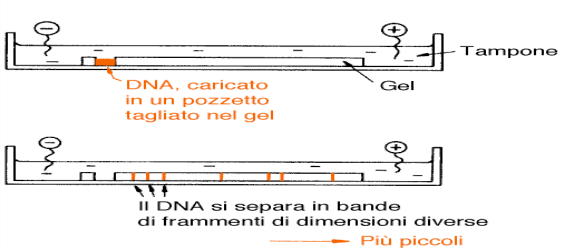
\includegraphics[width=0.6\textwidth]{./immagini/elettroforesi.png}
	\caption{Elettroforesi su GEL}
	\label{elettroforesi}

\end{figure}

\subsubsection{Materiali utilizzati}

\begin{itemize}
	\item Guanti in lattice
	\item Micropipette (100-1000 e 2-200 microlitri)
	\item Beuta da laboratorio
	\item Forno a micronde
	\item Strumenti per l'elettroforesi
	\item Eppendorf
\end{itemize}

\subsubsection{Soluzioni utilizzate}

\begin{itemize}

	\item Miniprep del pUC18
	\item Enzima di restrizione EcoR I
	\item Acqua
	\item Buffer 10X(digestione)
	\item TAE 50X
	\item SyberSafe
	\item Marker (DNA Ladder)

\end{itemize}

\subsection{Procedimento}

\subsubsection{Restrizione del DNA}

\begin{enumerate}

	\item prelevare \SI{10}{\micro\liter} di pUC18 e metterli in una nuova eppendorf
	ed altri \SI{11.5}{\micro\liter} da mettere in un'ulteriore eppendorf per effettuare in
	una provetta la reazione (con l'enzima) e nell'altra il controllo negativo (senza l'enzima).

	\item Addizionare alla eppendorf contenente il nostro plasmide,
	prima \SI{11.5}{\micro\liter} di H\textsubscript{2}O, successivamente
	\SI{2.5}{\micro\liter} di buffer 10X ed infine \SI{1}{\micro\liter} del nostro enzima di restizione EcoR I.

	\item Portare la eppendorf contenente la reazione ad una temperatura di 37°C
	(Temperatura ottimale per l'enzima di restrizione EcoR I) per 1-2 ore,
	in modo che l'enzima EcoR I possa compiere la sua catalizzazione.

\end{enumerate}

\subsubsection{Preparazione ed Elettroforesi}


\begin{enumerate}

	\item Per prima cosa si procede preparando il gel di agarosio 0.8\%, prendendo una beuta
	ed aggiungendo a questa 0.6 g di agarosio, 1.6 ml di TAE 50X e 78.4 ml di H\textsubscript{2}O
	in modo da avere un volume totale di 80 ml.

	\item La miscela a questo punto si presenterà con l'agarosio in fase solida,
	poichè a temperatura ambiente non è solubile.
	Dobbiamo perciò portare la soluzione ad una temperatura prossima all'ebollizione.
	Andremo quindi a scaldare il tutto all'interno di un forno a micronde, prestando attenzione
	che la soluzone non bolla per più di qualche secondo.

	\item Una volta estratta la beuta, facendo attenzione al calore,
	la si mescola fino a che non si otterrà una soluzione omogenea in contenuto e colore.

	\begin{figure}[H]
		\centering
		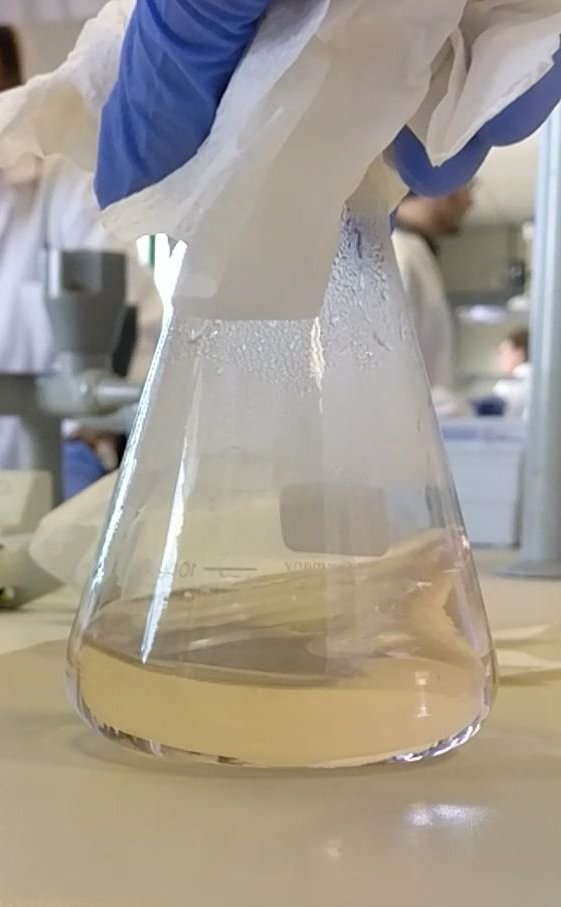
\includegraphics[width=0.3\textwidth]{./immagini/agarosio.jpg}
		\caption{Mescolamento della soluzione con agarosio}
		\label{agarosio}

	\end{figure}

	\item Una volta che la soluzione risulta omogenea e la sua temperatura \`e calata,
	si va ad aggiungere \SI{5}{\micro\liter} di SyberSafe.
	Questo serve come intercalante che si va a legare alla doppia elica
	e sottoposto a raggi UV si rende visibile grazie alla sua fluorescenza.

	\item Andiamo a versare la soluzione nella vaschetta apposita che,
	solidificandosi, ne prende la forma.
	Bisogna inserire il pettine all'interno della vaschetta,
	finch\`e il gel non ha ancora solidificato.
	In questo modo si creeranno i pozzetti dove si andrà a mettere il contenuto delle
	due eppendorf preparate in precedenza una volta che il gel risulter\`a solidificato.

	\begin{figure}[H]

		\centering
		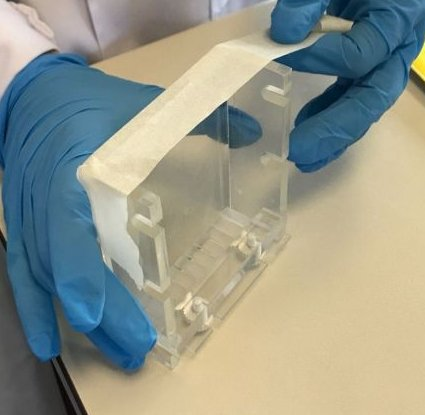
\includegraphics[width=0.3\textwidth]{./immagini/vaschetta.jpg}
		\caption{Vaschetta per solidificazione del gel di agarosio}
		\label{vaschetta}

	\end{figure}


	\item Non appena il gel si sarà solidificato, porlo nella vaschetta togliendo il pettine.
	\item Aggiungere 250 ml di buffer di corsa(TAE 1X) fino al livello indicato.
	\item Caricare all'interno dei pozzetti le varie soluzioni per la corsa elettroforetica tra cui:

	\begin{itemize}

		\item \SI{25}{\micro\liter} di pUC18 digerito (con \SI{5}{\micro\liter} di Loading Buffer)
		\item \SI{25}{\micro\liter} di pUC18 non digerito (con \SI{5}{\micro\liter} di Loading Buffer)
		\item \SI{25}{\micro\liter} di RNA totale derivante dalla scorsa esperienza
		(con \SI{5}{\micro\liter} di Loading Buffer)
		\item Un pozzetto è riservato per il Marker.

	\end{itemize}

	\begin{figure}[H]
		\centering
		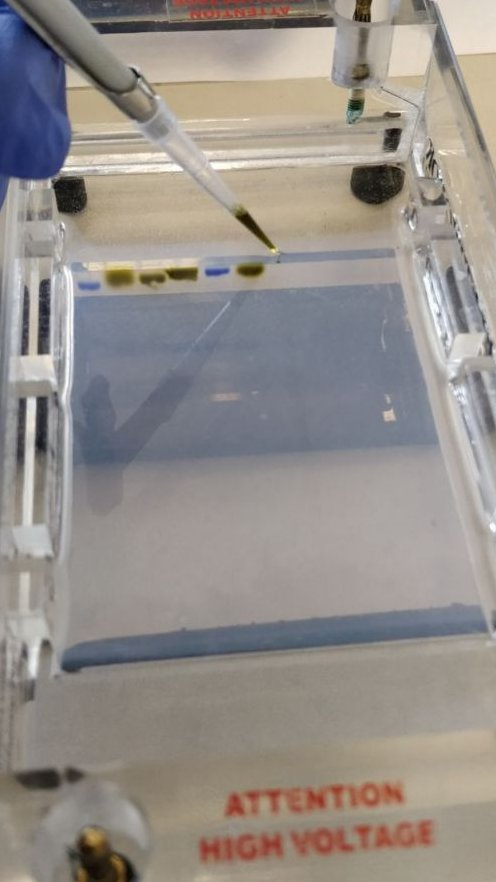
\includegraphics[width=0.3\textwidth]{./immagini/caricamento.jpg}
		\caption{Fase di caricamento dei pozzetti}
		\label{cricamento}
	\end{figure}

	Il Marker è un composto da una miscela di frammenti lineari di DNA con dimensioni
	note che migrano nel gel in prevedibile.
	In questo modo, \`e possibile confrontare il campione con il marker,
	determinando approssimativamente la lunghezza del frammento.

	Il Loading buffer è un colorante con velocità di migrazione nota,
	aggiunto ai composti inseriti nei pozzetti in modo da poter seguire
	l'andamento dell'elettroforesi.

	\begin{figure}[H]

		\centering
		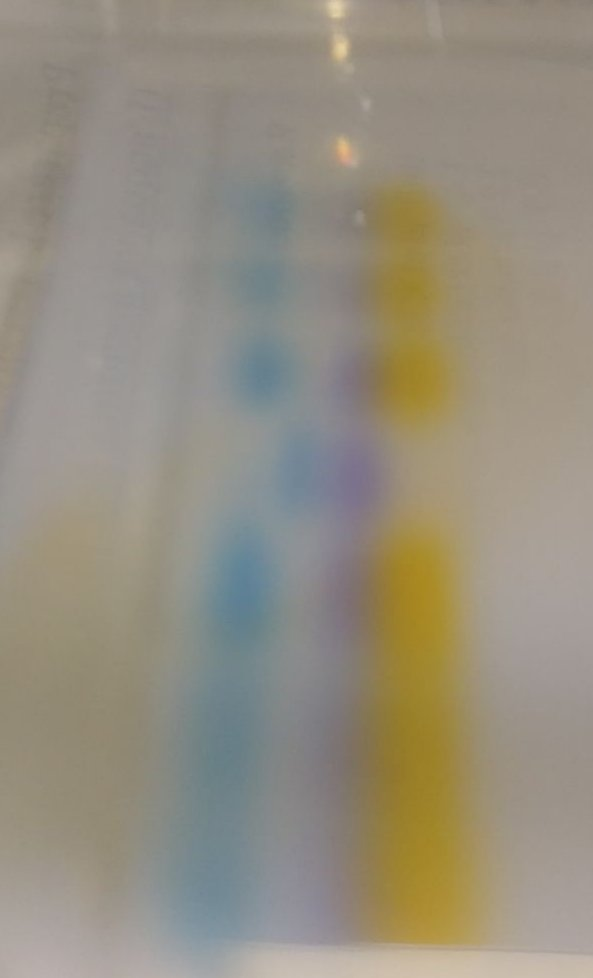
\includegraphics[width=0.3\textwidth]{./immagini/separazione.jpg}
		\caption{Divisione delle bande colorate (Loading buffer)}
		\label{loading_buffer}

	\end{figure}

	\item Caricati i pozzetti chiudere la scatola per l'elettroforesi ed azionare la corrente,
	aspettando il tempo necessario affinch\`e bande risultino ben separate.

	\item Finita la corsa elettroforetica, prendere il gel e metterlo su una piastra
	che emana raggi UV. Coprire con una lastra di vetro che non permetta la fuoriuscita dei raggi UV,
	in modo da non danneggiare gli occhi.
	Avviare la macchina che emette radiazioni UV, in modo da vedere le bande dove il DNA \`e localizzato.
	Confrontandolo con le bande del marker, si pu\`o capire la lunghezza dei vari frammenti.

	\begin{figure}[H]

		\centering
		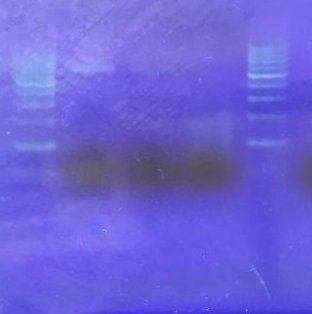
\includegraphics[width=0.3\textwidth]{./immagini/uv.jpg}
		\caption{Fluorescenza del SyberSafe (DNA)}
		\label{SyberSafe}

	\end{figure}



\end{enumerate}


\subsection{Risultati e Conclusioni}

Durante questa esperienza abbiamo capito il funzionamento dell'elettroforesi nei suoi passaggi,
tra cui la preparazione del gel di agarosio, la preparazione e la colorazione delle soluzioni,
il caricamento nei pozzetti di queste e la successiva fluorescenza data dai raggi UV.

Abbiamo compreso poi il processo di digestione tramite gli enzimi di restrizione,
nel nostro caso l'enzima EcoR I.

Andando a guardare l'immagine risultante dalla fluorescenza,
possiamo notare come nei nostri pozzetti,
la quantità di DNA è molto bassa rispetto al
marker (all'interno del primo pozzetto e del sesto pozzetto).
Questo può essere causato da una poca quantità di materiale, oppure qualche errore nella procedura.
Confrontando con le bande del marker possiamo capire all'incirca le dimensioni dei nostri frammenti.

	\newpage
	%_______________________________ESPERIENZA N° 6 (XL1_BLUE)
	\section{\LARGE{Trasformazione delle cellule di escherichia coli xl1 blue}}

\vspace{0.6cm}

\subsection{Sommario}

\subsubsection{Scopo}

L'obiettivo di questa esperienza è quello di manipolare le \textbf{culture batteriche di E.coli}
(batterio gram negativo non patogeno usato comunemente nei laboratori di ricerca),
andando a \textbf{trasportare il plasmide pUC18}, precedentemente trattato,
all'interno di questi batteri diventando cos\`i un ceppo di propagazione
(atto al clonaggio e alla propagazione di plasmidi) all'interno di un terreno di crescita.

\subsubsection{Cenni teorici}

Il procedimento di trasporto del dsDNA da esterno alla cellula all'interno è chiamato
\textbf{trasformazione batterica}, ed è un fenomeno parasessuale che consente ai batteri
lo scambio di materiale genico.

Solo alcune specie batteriche possono acquisire DNA estraneo dall'ambiente (DNA esogeno)
che deve essere a doppia elica, con facilità.
Queste sono dette cellule \textit{"naturalmente competenti"}.
Altre specie invece diventano competenti solo in particolari condizioni fisiologiche
ed altre ancora, come per esempio E.coli, necessitano di una trasformazione artificiale in
laboratorio tramite vari metodi chimici o fisici
(da noi usato è il metodo dello \textit{shock-termico}) che le rende \textbf{competenti}.

Una volta che il plasmide si trova all'interno della cellula batterica di E.coli,
la si fa crescere all'interno di piastre precedentemente preparate con LB-agar-amp
(Luria Bertani medium with ampicillin), in grado di fornire il nutrimento necessario
alla cellula per potersi nutrire e clonare,
producendo molte copie contenenti molti plasmidi ingegnerizzati di nostro interesse.

\subsection{Materiali utilizzati}

\begin{itemize}
	\item Guanti in lattice
	\item Provette Eppendorf (2mL)
	\item Micropipette (100-1000  e 2-200 microlitri  )
	\item Scatola di polistirolo contenente ghiaccio
	\item Bagno termostatico
	\item Piasra di LB-agar-amp
	\item Bacchette in vetro
\end{itemize}

\subsection{Soluzioni utilizate}

\begin{itemize}
	\item Miniprep del pUC18
	\item Cellule competenti
	\item LB liquido
\end{itemize}

\subsection{Procedimento}

\begin{enumerate}
	\item Diluire la nostra miniprep del pUC18 (descritta nell'esperienza numero 1)
  in acqua pura in misura 1:10 quindi prelevare 1$\mu$l di miniprep del pUC18 e
  9$\mu$l di acqua pura tramite una micropipetta e inserire le due componenti
  in una nuova provetta eppendorf da 2 ml. \\
  Questa diluizione \`e necessaria per avere un totale di 10$\mu$l.


	\item Prelevare in un \textit{ambiente biologicamente sterile} (sotto cappa biologica) 100 microlitri
  di cellule competenti e metterli in una provetta eppendorf da 2 ml.
  Lavorando in un ambiente sterile si garantisce la protezione da agenti inquinanti derivanti dall’esterno.

	\item Aggiungere 1$\mu$l della miniprep, diluita con acqua al passo n° 1,
  all'interno della eppendorf contenente le cellule competenti.
  In questo modo si forma una soluzione sia di cellule batteriche che di plasmidi,
  che dovranno poi entrare all'interno delle cellule.

	\item Agitare la soluzione per far s\`i che i plasmidi si distribuiscano in
  modo uniforme.
  \item Incubare la provetta contenente la soluzione in ghiaccio per una trentina di minuti
  in modo che la temperatura si abbassi gradualmente di qualche grado e che i plasmidi
  si vadano a legare sulla membrana della cellula batterica.

	\item Attendere 30' in modo che la temperatura della soluzione contenente cellule e plasmidi si è abbassi
  e stabilizzi.
  \item Ora linea teorica i plasmidi sono ancorati alle membrane delle cellule dove dovranno poi essere
  incorporati.
  \item A questo punto effettuare lo \textbf{shock termico}, portando la provetta eppendorf
  da una temperatura di ca. 0°C(ghiaccio) ad una temperatura di 42°C  molto rapidamente e lasciarla
  nel bagno termostatico per 1 minuto (la tempistica è importante poichè se si lascia il tutto ad una
  temperatura elevata per troppo tempo le cellule batteriche potrebbero morire).
  Questa operazione \`e di cruciale importanza, infatti fa in modo che sulle membrane delle cellule batteriche
  di E.coli si \textit{aprano dei pori}, permettendo il passaggio del DNA esogeno (plasmide) all'interno
  formando così una \textbf{cellula trasformata}.
	Un altro metodo per effettuare l'apertura dei pori e la successiva immissione dei plasmidi all'interno
  delle cellule competenti è l'elettroporazione che consiste in una repentina scarica elettrica
  ad alto voltaggio. Il vantaggio di questa tecnica \`e che può essere applicata anche a cellule eucariotiche.

	\begin{figure}[H]
		\centering
		\subfloat{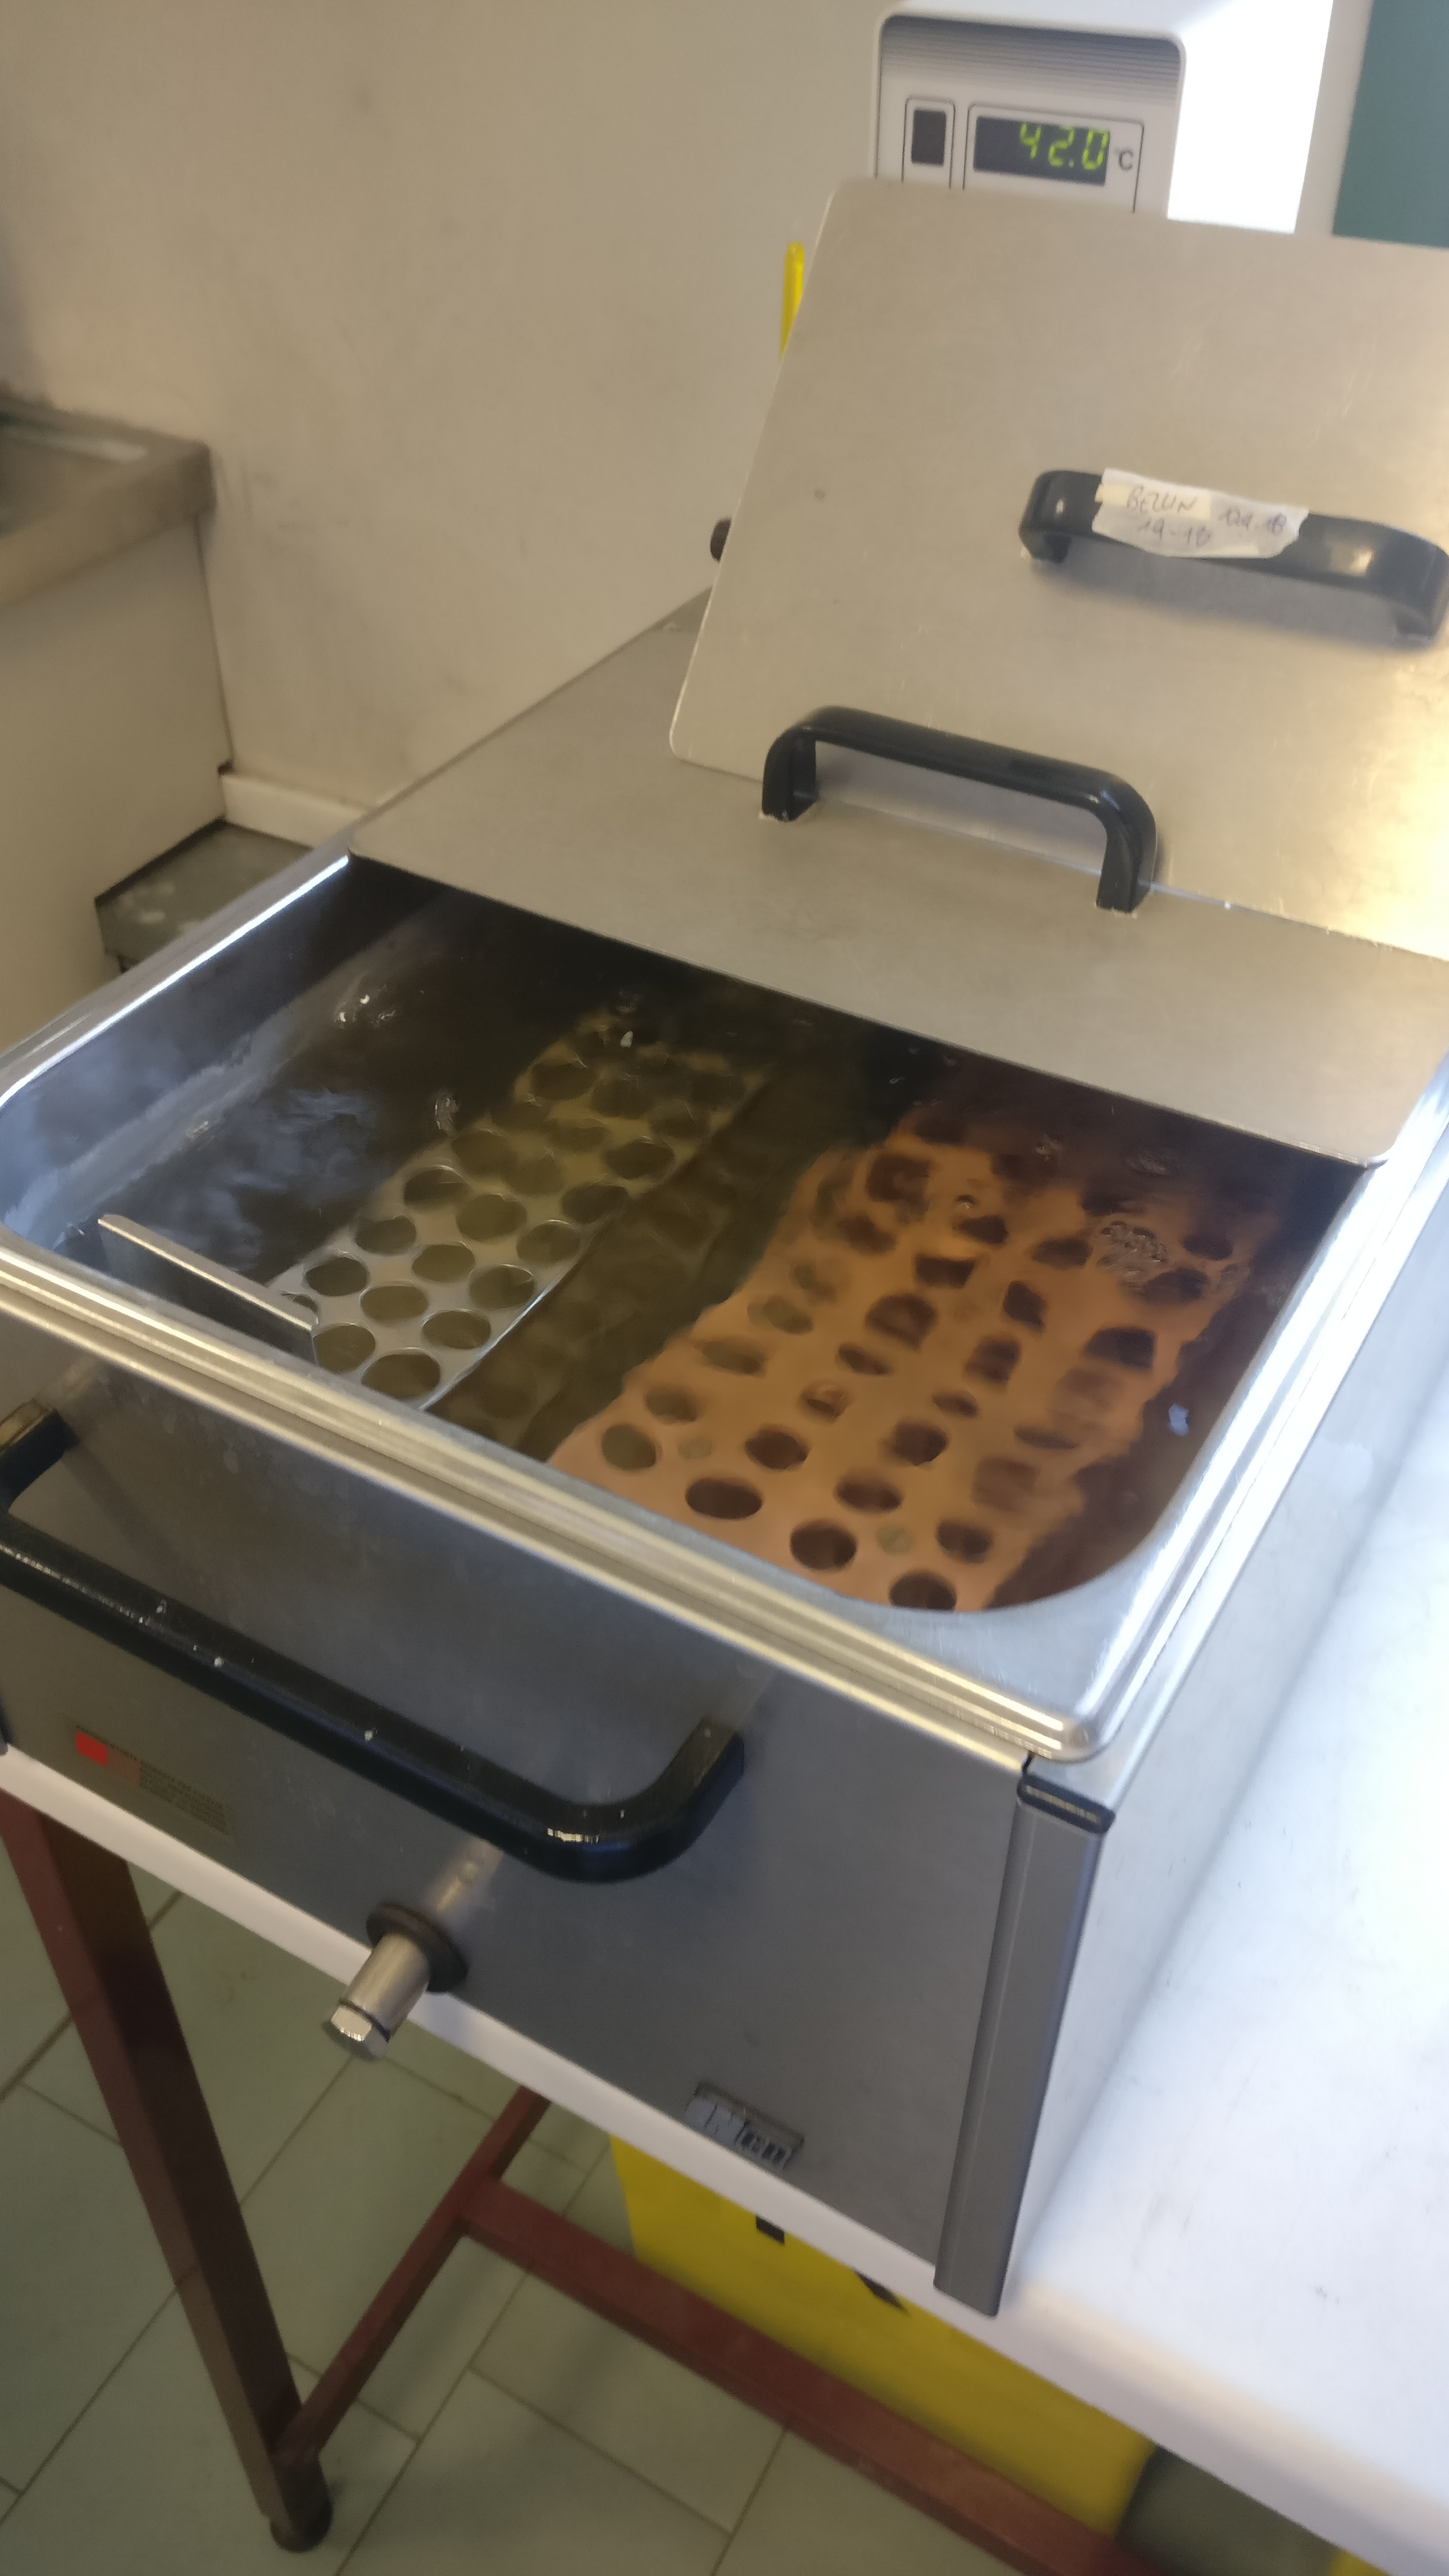
\includegraphics[width=0.3\textwidth]{./immagini/bagno_termostatico.jpg}} \quad
		\subfloat{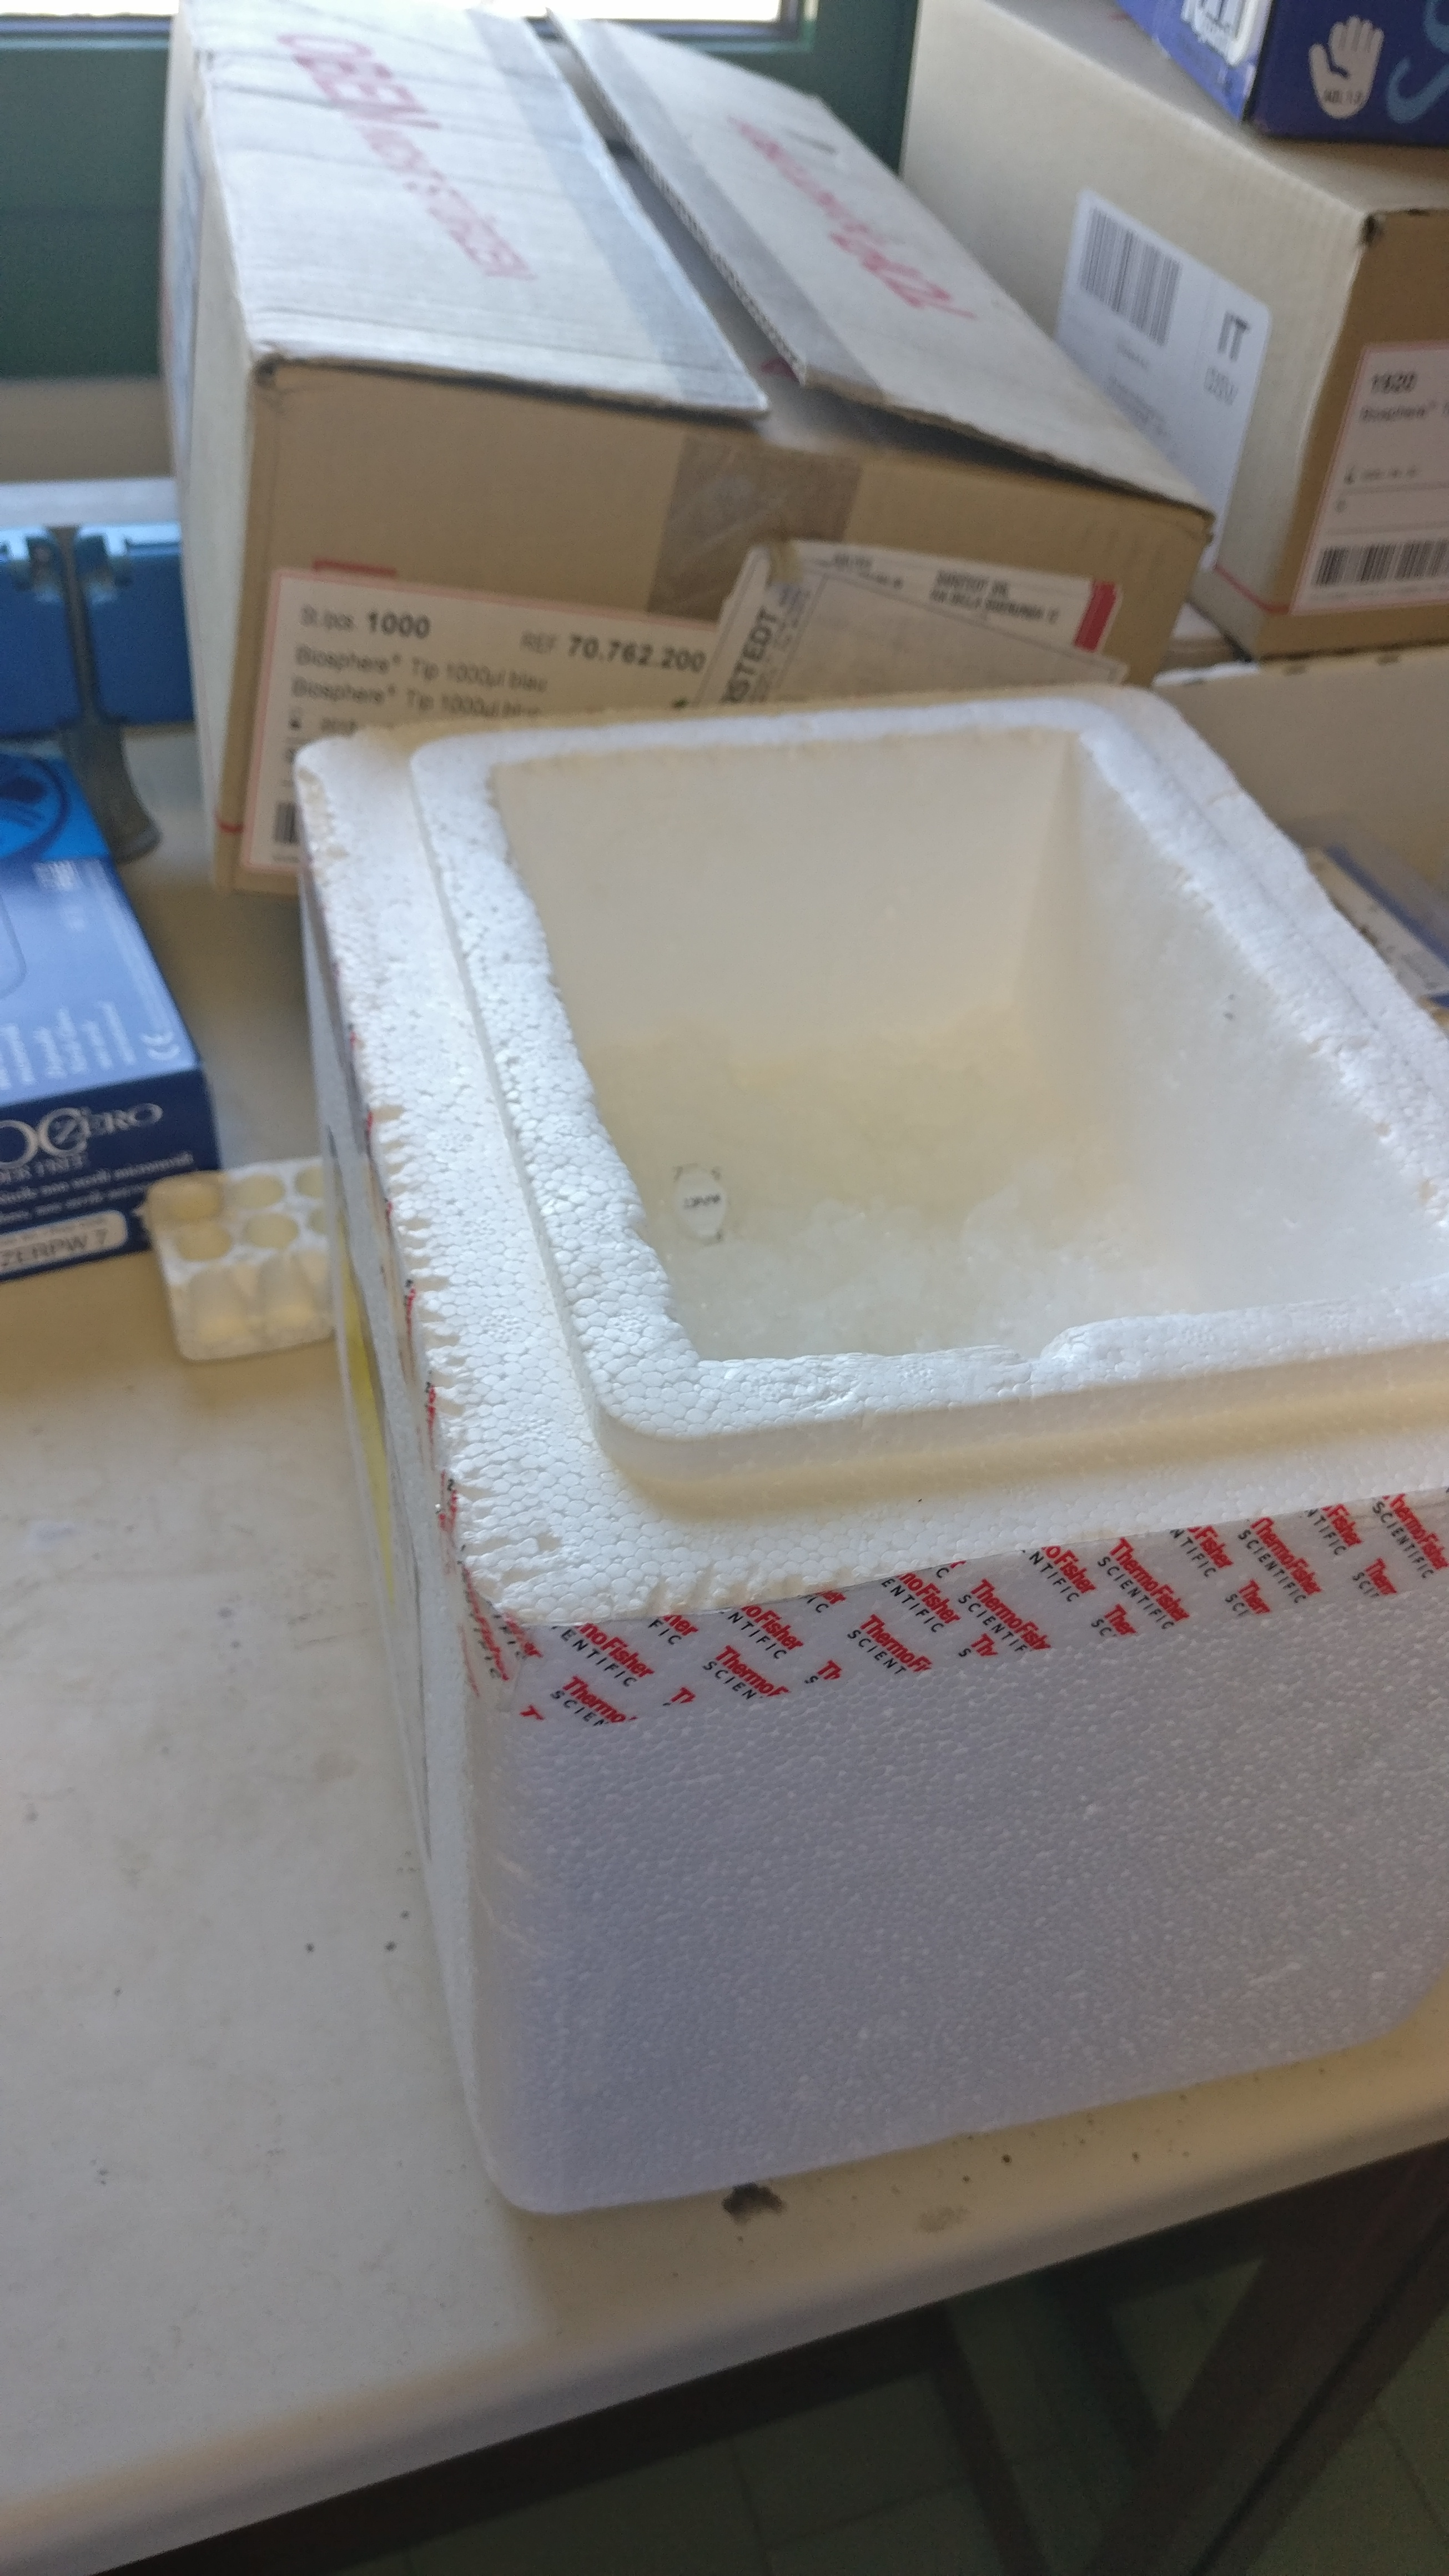
\includegraphics[width=0.3\textwidth]{./immagini/ghiaccio.jpg}}
		\caption{Bagno termostatico e immersione in ghiaccio}
		\label{bagno_e_ghiaccio}
	\end{figure}
	\item Passato un minuto prendere la eppendorf e rimetterla in ghiaccio per altri 5 minuti,
  favorendo il \textit{rallentamento del metabolismo cellulare}.
	\item Aggiungere del nutriente LB liquido all'interno della provetta, e incubarla a 37°C per 1 ora.
   In questo modo la cultura batterica si accresce e si esprime la \textbf{resistenza all'antibiotico}
   (ampicillina, codificata dal gene contenuto all'interno del plasmide).
    Una volta messo sul terreno di LB-amp, questo ci permette di sapere se il nostro plasmide è
    stato effettivamente incorporato all'interno della cellula batterica o no.
	\vspace{0.3cm}

	\begin{figure}[H]

		\centering
		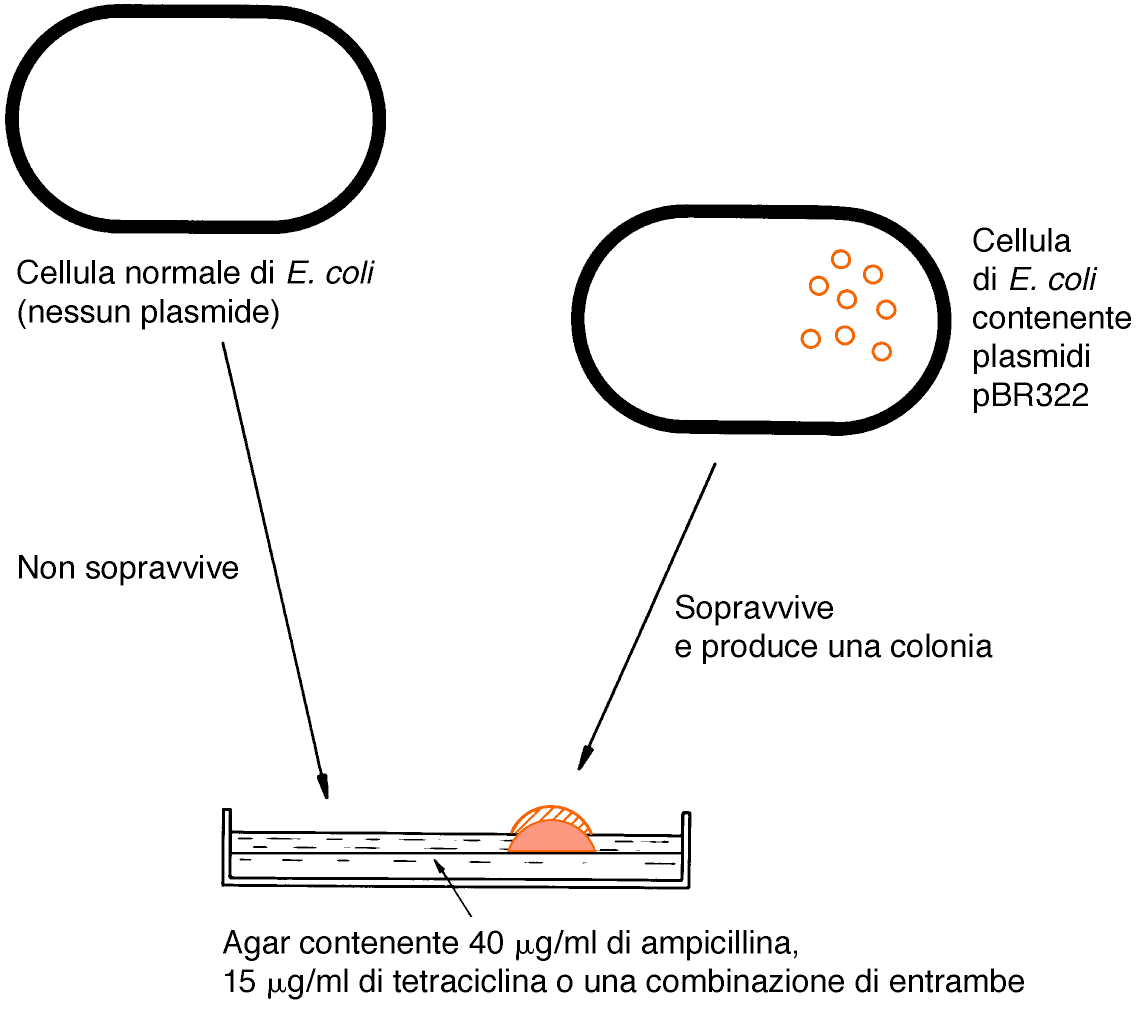
\includegraphics[width=0.6\textwidth]{./immagini/resistenza_ampicillina.png}
		\caption{Colonie con il plasmide integrato resistono al terreno con ampicillina }
		\label{resistenza ampicillina}

	\end{figure}

	\item Piastrare 150-200 microlitri della sospensione delle cellule su di una piastra di LB-amp,
  distribuendole con una bacchetta di vetro a forma di 'L' su tutta la superficie.
  Metterle poi ad una temperatura di 37°C per una notte a crescere.

	\begin{figure}[H]
		\centering
		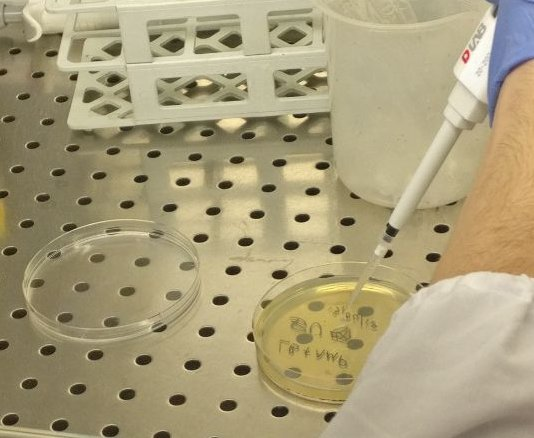
\includegraphics[width=0.6\textwidth]{./immagini/piastraggio_colonie.jpg}
		\caption{Piastraggio delle cellule di E. Coli su terreno LB-Amp}
		\label{piastraggio cellule}
	\end{figure}
\end{enumerate}

\subsection{Risultati e Conclusioni}

Tramite questa procedura abbiamo potuto inserire all'interno delle nostre cellule batteriche
di E.coli i plasmidi pUC18 rendendole competenti, permettendoci cos\`i di clonare od esprimere
i geni di interesse.

	\newpage
	%_______________________________ESPERIENZA N° 12 (SEPARAZIONE CELLULARE SU GRADIENTE DI FICOLL)
	\chapter{Separazione cellulare su gradiente di ficoll}

\vspace{0.6cm}

\section{Sommario}

\subsection{Scopo}

In questa esperienza introduciamo la metodologia di separazione per le cellule del sangue.
Questa operazione viene effettuata per purificare linfociti e monociti,
separandoli dai globuli rossi e dai granulociti (esempio piastrine) che sono di gran
lunga i componenti più numerosi del sangue.\\
Considerazione: essendo che non possiamo lavorare con il sangue in quanto può
essere molto rischioso abbiamo usato delle cellule di melanoma prese da una coltura.


\subsection{Cenni teorici}
Questa procedura viene usata specialmente per il sangue.
Essa permette di isolare le sue diverse componenti in modo tale da poter successivamente
lavorare più nello specifico con quelle di nostro interesse.\\
Un ruolo importante lo riveste il Ficoll.
Il Ficoll è un copolimero sintetico di alto peso molecolare e grazie alla sua densità
permette di spingere verso il fondo quelle componenti che non ci interessano.
Quindi nel caso del sangue otterremo 4 diverse fasi:
\begin{figure}[H]
    \centering
    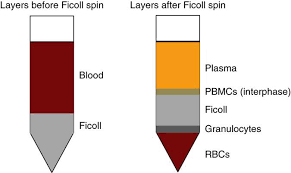
\includegraphics{./immagini/Ficoll_sangue.png}
    \caption{Falcon con sangue pre e post centrifuga}
\end{figure}

\section{Materiali utilizzati}

\begin{itemize}
\item Guanti in lattice
\item Provette Eppendorf (1.5 mL)
\item Falcon da 15 ml
\item Falcon da 50ml
\item Camera di Burker
\item Centrifuga
\item Micropipetta (\SI{100}{\micro\liter}-\SI{1000}{\micro\liter})

\end{itemize}

\section{Soluzioni utilizzate}

\begin{itemize}

\item PBS
\item Tripsina
\item Wash Buffer (terreno di coltura contenente FBS)
\item FBS
\item Ficoll

\end{itemize}

\section{Procedimento}

\subsection{Preparazione della sospensione cellulare}

\begin{enumerate}

    \item Eliminare il terreno di coltura

    \item Lavare le cellule con 20 ml di PBS; eliminare il liquido di lavaggio

    \item Ripetere il lavaggio con ulteriori 20 ml di PBS; eliminarlo

    \item Addizionare 5 ml di tripsina; lasciare incubare per 5' a 37°C.
    La tripsina permette di staccare le cellule in modo non meccanico (senza cell scraper).

    \item Addizionare alla tripsina 15 ml di Wash Buffer (terreno di coltura con FBS).

    \item Centrifugare a 300g per 10' RT.

    \item Risospendere in 50 ml di Wash Buffer.

    \item A 5 ml di sospensione aggiungere ulteriori 5 ml di Wash Buffer portando
    ad un volume di 10 ml totali.

\end{enumerate}

\subsection{Allestimento separazione su gradiente}

\begin{enumerate}
    \item Diluire il PBS 10X e prelevarne 50 ml 1X in una falcon da 50 ml.
    \item Aliquotare su una Falcon da 15 ml 4 ml di Ficoll.
    \item Stratificare molto lentamente, mediante l'utilizzo di una Pasteur monouso,
    la sospensione di cellule; bisogna far attenzione a non agitare per non compromettere
    la stabilità della deposizione su Ficoll.
    \item Centrifugare per 30' a 800 g RT senza accelerazione nè freno.
    \item Dopo la centrifuga si ottiene una separazione su gradiente che isolerà le cellule
    formando un anello in base alla loro densità. Otteniamo nel nostro caso solo una fase,
    ma nel caso del sangue si vedrebbero diverse fasi che rappresentano le varie componenti.
    \item Prelevare l'anello di cellule formatosi tra il Ficoll e il liquido si sospensione
    cellulare facendo particolare attenzione in quanto è un passaggio delicato.
    Prelevato l'anello spostarlo in una Falcon da 15 ml.
    \item Riempire per decantazione la Falcon di PBS portandolo a un volume finale di 15 ml.
    \item Centrifugare a 400g per 10'; finita la centrifuga scartare il surnatante
    e risospendere il pellet di cellule.
    \item Aggiungere per decantazione ulteriore PBS e portarlo a un volume di 10 ml.
    \item Centrifugare nuovamente a 400 g per 10'; finita la centrifuga scartare di nuovo
    il surnatante e risospendere in 1ml di PBS con la micropipetta da 100 $\mu$.
    \item Spostare infine su una eppendorf da 1.5 ml.
\end{enumerate}

\subsection{Conta cellulare su camera contaglobuli di Burker}
\begin{enumerate}
    \item Diluire le cellule 1:10 in $\mu$ finali su nuova eppendorf.
    \item Montare la camera di Burker.

    \begin{figure}[H]
    \centering
    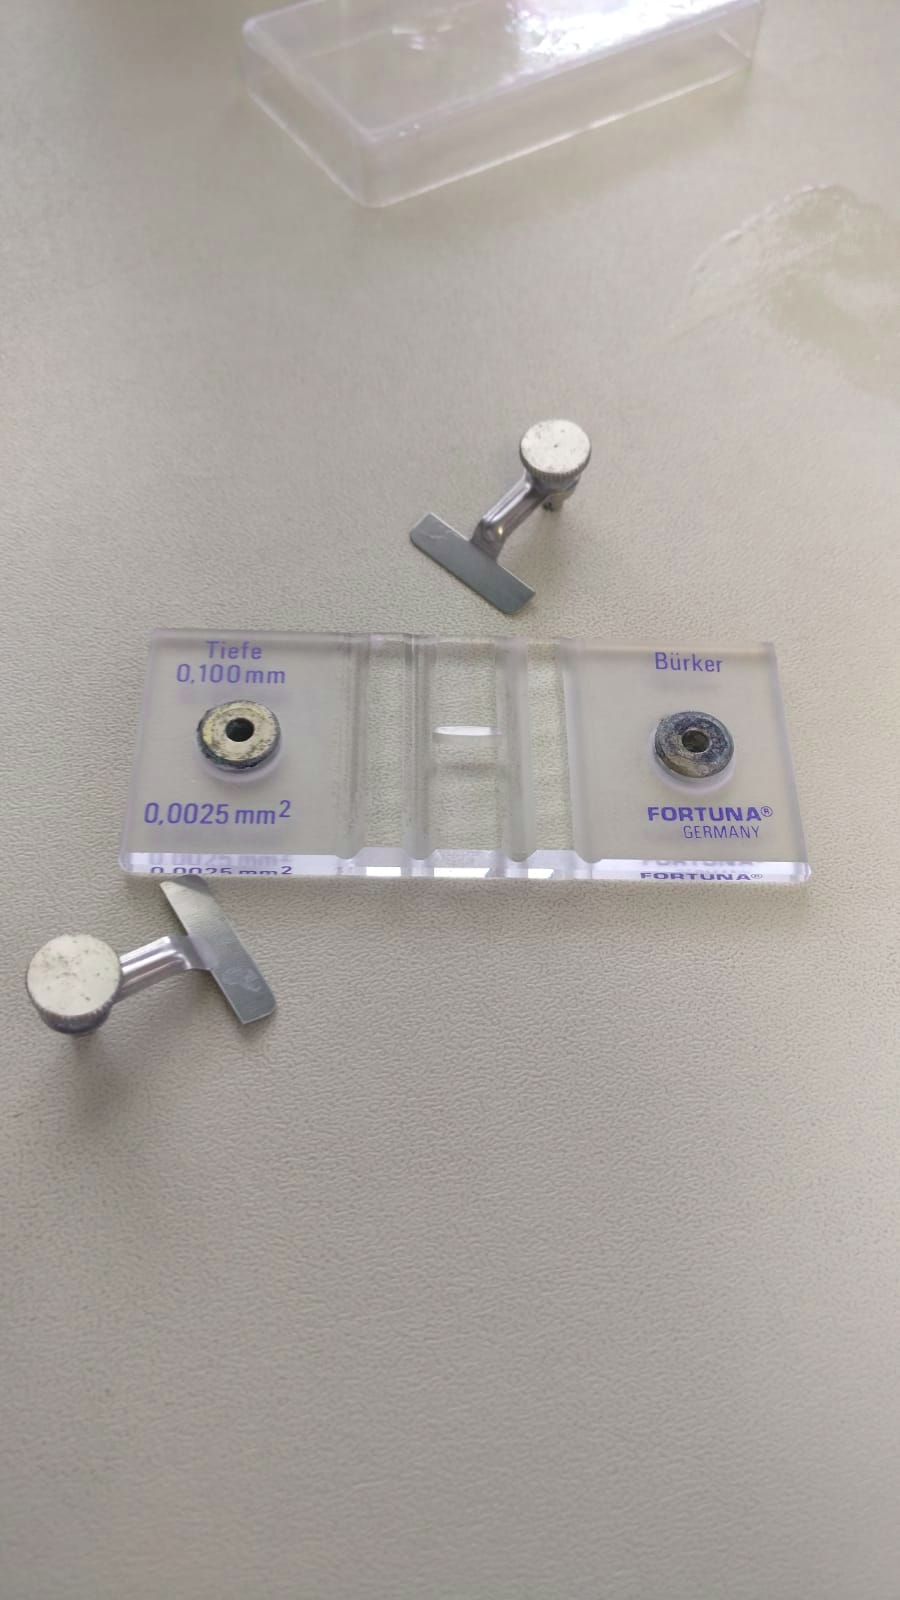
\includegraphics[width = 0.4\textwidth]{./immagini/Burker.png}
    \caption{Burker}
    \end{figure}

    \item Riempire i due pozzetti della camera per capillarità mediante l'utilizzo di
    una pipetta da 200 $\mu$l. Capiamo che la camera è piena quando da sotto il
    copri-vetrino uscirà una goccia.
    \item Contare le cellule comprese all'interno del quadrato che presenta come bordo 3
    righe.
\end{enumerate}

\section{Risultati e Conclusioni}

Il numero di cellule da noi trovate è 92. Un numero così elevato è stato ottenuto per la
non diluizione specificata precedentemente. \\
Il totale delle cellule diluite si sarebbe ottenuto con questa formula :
    $$[cellule] = (num. cellule)*(fatt. diluzione)*(fatt. moltiplicativo camera)$$
Nel nostro caso il fattore moltiplicativo della camerà è 10000.

\end{document}

	\newpage

	



\end{document}
